\documentclass{article}
\usepackage{graphicx} % Required for inserting images
\usepackage[utf8]{inputenc} % Encodage du document
\usepackage[T1]{fontenc} % Encodage des caractères
\usepackage[margin=1.75cm,headheight=1cm,headsep=2.5mm]{geometry} % Marges du document
\usepackage{hyperref} % Hyperliens
\usepackage{xcolor} % Couleurs
\usepackage{titlesec} % Définition des titres
\usepackage{fancyhdr}
\usepackage{tcolorbox}
\usepackage{stmaryrd}
\usepackage{float}
\usepackage{amsmath}
\usepackage{amsthm}
\usepackage{amsfonts}
\usepackage{multicol}
\usepackage{pgf}
\usepackage{esint}
\usepackage{appendix}
\usepackage[english]{ babel} % Langue du document
\usepackage[sorting=none]{ biblatex} % Bibliographie
% Definition de la bibliographie
\addbibresource{Biblio/biblio.bib} % Lien vers le fichier créé précedemment
\usepackage{pdfpages}
\usepackage{tkz-euclide}
% \usepackage{listings}
\usepackage{float}
\usepackage{enumitem}
\usepackage{xcolor}
\usepackage{placeins}
\usepackage{caption}
\usepackage{lastpage}
\usepackage[T1]{fontenc}
\usepackage{tocloft}
\usepackage{tikz}
\usepackage{bm}
\usepackage{subcaption}

\setlength{\hoffset}{-15pt} 

\setlength{\parindent}{0pt}

\usepackage{pgfplots}
\pgfplotsset{compat=1.18}

% Hyperref : définition des couleurs des liens et des citations
\hypersetup{
    citecolor=red, % Couleur des citations
    colorlinks=true, % Activer les liens colorés
    linkcolor=blue, % Couleur des liens
    urlcolor=bleuPonts, % Couleur des liens vers des URL
    pdfpagemode=FullScreen, % Mode plein écran par défaut
}


\theoremstyle{definition} 
\newtheorem{defi}{Definition}[section] 
\theoremstyle{proposition}  
\newtheorem{prop}{Proposition}[section] 
\theoremstyle{theorem} 
\newtheorem{thm}{Theorem}[section] 
\theoremstyle{remark}
\newtheorem{rmk}{Remark}[section] 
\theoremstyle{corollary}  % makes text upright (not italic)
\newtheorem{cor}{Corollary}[section] 

\newtheoremstyle{exercise}
  {3pt}   % Space above
  {3pt}   % Space below
  {\normalfont} % Body font (normal color)
  {}      % Indent amount
  {\color{red}\bfseries} % Head font (red)
  {.}     % Punctuation after head
  { }     % Space after head
  {} 
\theoremstyle{exercise}  
\newtheorem{exo}{Exercise}[section] 
\theoremstyle{lemma} 
\newtheorem{lem}{Lemma}[section] 

\setcounter{page}{1}
\pagestyle{fancy}
\fancyhead{}
\lhead{{HOULETTE} \\ {\typeRapport}}
\chead{\textsc{ \sousTitre}}
\rhead{\dateRapport}
\fancyfoot{}
\fancyhf{}
\fancyfoot[C]{\thepage}

\renewcommand{\cftsecleader}{\cftdotfill{\cftdotsep}}

\newcommand{\vb}[1]{\bm{#1}}

\usepackage{minted}
\captionsetup[lstlisting]{labelfont=bf, labelsep=colon, name=Figure}
\usemintedstyle{vs} 

% Global minted options
\setminted{
  frame=lines,
  framesep=6pt,
  baselinestretch=1.0,
  linenos,
  numbersep=6pt,
  fontsize=\footnotesize,
  breaklines=true
}


%\newpage
\title{\textbf{Project Report : $\mathbb{P}_2$-Lagrange finite elements}}
\author{Maxime Houlette}
\date{}

\begin{document}

\maketitle
\vspace{3cm}

{\hypersetup{linkcolor=black}
\tableofcontents}

\newpage

\section{Short introduction to $\mathbb
P_2$-Lagrange finite elements}

The goal of this section is to provide a short reminder of what $\mathbb P_2$-Lagrange finite elements are, and what the main differences are with $\mathbb P_1$-Lagrange finite elements. \\

\subsection{$\mathbb P_k$-Lagrange finite elements}

Given a conforming mesh $\mathcal{T}_h$, we recall that for all $K \in \mathcal{T}_h$, the $\mathbb P_k$-Lagrange finite element is the simplicial finite element defined as follows:

$$(K, \, \mathcal{P}_K, \, \Sigma_K)$$

such that : 

\begin{itemize}
    \item[$\bullet$] $K$ is a $d$-simplex
    \item[$\bullet$] $\mathcal{P}_K$ is the set $\mathbb P_k(K)$ (polynomials of total degree $k$), which has the dimension $\binom{d+k}{d}$
    \item[$\bullet$] $\Sigma_K$ is the set of the linear forms associated to the evaluation of an element of  $\mathcal{P}_K$ over the vertices of the principle lattice of order $k$.
\end{itemize}

We introduce the principal lattice of order $k$ associated to a simplex $K$

$$T_k(K) = \Big\{\bm x\in \mathbb{R}^d: \lambda_j(\bm x) \in \{0, \, \frac{1}{k}, \, \dots, \, \frac{k-1}{k}, \, 1\}, \, \forall j \in \llbracket 1, d+1\rrbracket\Big\} = (\bm x_i)_{1\leq i \leq \binom{d+k}{d}}$$

where the $\lambda_j(\bm x)$ are the barycentric coordinates of $\bm x$ in the simplex $K$. Then 

$$\Sigma_K = (\sigma_i)_{1\leq i \leq \binom{d+k}{d}}$$

where 

$$\forall p \in \mathcal{P}_K, \, \sigma_i(p) = p(\bm x_i)$$

The unisolvence property is satisfied, so this is a well-posed finite element. Denoting $\Phi$ the isomorphism

\[
\vcenter{\hbox{$\Phi$}}
\;:\;
\begin{aligned}
\mathcal{P}_K &\to \mathbb{R}^{\binom{d+k}{d}} \\
p &\mapsto \left(p(\bm x), \dots, p(\bm x_{\binom{d+k}{d}})\right)
\end{aligned}
\]

and considering the canonical basis of $\mathbb{R}^{\binom{d+k}{d}}$, we build a basis of $\mathcal{P}_K$ by considering its unique preimage by $\Phi$, that we denote $(\varphi_i)_{1\leq i \leq \binom{d+k}{d}}$. Hence, this basis of $\mathcal{P}_K$ satisfies 

$$\forall (i, j) \in \llbracket 1, \binom{d+k}{d} \rrbracket^2, \, \varphi_i(\bm x_j) = \delta_{ij}$$

\subsection{Particular case $d=2$ and $k=2$}

In the case where $d=2$ and $k=2$, for all $K \in \mathcal{T}_h$, we are considering $\mathcal{P}_K = \mathbb P_2(K)$, which has the dimension $6$. In that case, the principle lattice of order $2$ of a given $K$ is 

$$T_2(K) = \Big\{\bm x\in \mathbb{R}^d: \lambda_j(\bm x) \in \{0, \, \frac{1}{2}, \, 1\}, \, \forall j \in \llbracket 1, 3\rrbracket\Big\} = \{\bm x_1, \bm x_2, \bm x_3, \bm x_{12}, \bm x_{23}, \bm x_{31}\}$$

The points $(\bm x_1, \bm x_2, \bm x_3)$, which are the mesh vertices, and $(\bm x_{12}, \bm x_{23}, \bm x_{31})$, the edge midpoints, can be represented as follows:

\begin{figure}[H]
\label{fig:tri}
\begin{center}
\begin{tikzpicture}[scale=3]

\coordinate (x1) at (0,0);
\coordinate (x2) at (1.6,-0.3);
\coordinate (x3) at (0.6,0.8);

\draw[thick] (x1) -- (x2) -- (x3) -- (x1);

\foreach \p in {x1,x2,x3} {
    \fill[black] (\p) circle (1.5pt);
}

\coordinate (y1) at ($(x1)!0.5!(x2)$);
\coordinate (y2) at ($(x2)!0.5!(x3)$);
\coordinate (y3) at ($(x3)!0.5!(x1)$);

\foreach \m in {y1,y2,y3} {
    \draw[black, thick] (\m) ++(-1.5pt,-1.5pt) -- ++(3pt,3pt);
    \draw[black, thick] (\m) ++(-1.5pt,1.5pt) -- ++(3pt,-3pt);
}

\node[left=2mm]  at (x1) {$\bm x_1$};
\node[right=2mm] at (x2) {$\bm x_2$};
\node[above=2mm] at (x3) {$\bm x_3$};
\node[below=2mm] at (y1) {$\bm x_{12}$};
\node[right=2mm] at (y2) {$\bm x_{23}$};
\node[left=2mm]  at (y3) {$\bm x_{31}$};

\end{tikzpicture}
\caption{Local simplex $K$}
\end{center}
\end{figure}

We are now interested in computing the $\varphi_i$. It is clear that the main challenge of this framework will be handling the fact that the vertices are no longer the only degrees of freedom, as mid-edge points have been added.

\subsection{Shape functions}

We compute the $\mathbb{P}_2$ shape functions associated with the triangle $K$ shown in Figure 1. We provide the computational details for the shape function associated with $\bm x_1$ in barycentric coordinates, denoted as $\tilde{\varphi}_{\bm x_1}$. \\

By definition, $\tilde{\varphi}_{\bm x_1} \in \mathbb{P}_2(\hat{K})$ is uniquely determined by the following six constraints:

$$1 = \underbrace{\tilde{\varphi}_{\bm x_1}(1, 0)}_{\varphi_{\bm x_1}(\bm x_1)}$$

and 

$$0 = \underbrace{\tilde{\varphi}_{\bm x_1}(0, 1)}_{\varphi_{\bm x_1}(\bm x_2)} = \underbrace{\tilde{\varphi}_{\bm x_1}(0, 0)}_{\varphi_{\bm x_1}(\bm x_3)} = \underbrace{\tilde{\varphi}_{\bm x_1}\left(\frac{1}{2}, \frac{1}{2}\right)}_{\varphi_{\bm x_1}(\bm x_{12})} = \underbrace{\tilde{\varphi}_{\bm x_1}\left(0, \frac{1}{2}\right)}_{\varphi_{\bm x_1}(\bm x_{23})} = \underbrace{\tilde{\varphi}_{\bm x_1}\left(\frac{1}{2}, 0\right)}_{\varphi_{\bm x_1}(\bm x_{31})}$$

Solving a linear system of six equations yields 

$$\tilde{\varphi}_{\bm x_1}(\lambda_1, \lambda_2) = \lambda_1(2\lambda_1 - 1)$$

We end up with the table : 

\begin{table}[H]
\centering
\begin{tabular}{|c|c|c|}
\hline
 & $\bm z = \bm x_i$ & $\bm z = \bm x_{i \bar{i}}$ \\
\hline
$\tilde{\varphi}_{\bm z}(\lambda_1, \lambda_2)$
& $\lambda_i(2\lambda_i - 1)$  & $4\lambda_i\lambda_{i+1}$ \\
\hline
\end{tabular}
\caption{Reference $\mathbb{P}_2$ shape functions}
\end{table}

with the notation $\bar{i} = i+1$ and the conventions $\lambda_4 = \lambda_1$ and $\bm x_{34} = \bm x_{31}$.

\section{Local mass and stiffness matrices}

Given a triangle $K = (\bm x_1, \, \bm x_2, \, \bm x_3)$, we will extensively use the fact that 

$$\bm x\in K \Leftrightarrow \lambda_j(\bm x) \geq 0 \ \text{and} \ \sum_{i=1}^3\lambda_j(\bm x)=1$$

Considering the reference triangle $\hat{K} := ((0, 0), \, (1, 0), \, (0, 1))$, every $\bm x\in K$ can be uniquely represented with $(\lambda_1(\bm x), \lambda_2(\bm x)) \in \hat{K}$ (as $\lambda_3(\bm x) = 1 - \lambda_1(\bm x) - \lambda_2(\bm x)$). \\

For a function $f$ defined on a triangle $K$, the integral over $K$ can be computed using the change of variables $\bm x \in K \leftrightarrow (\lambda_1(\bm x), \lambda_2(\bm x)) \in \hat{K}$, which yields:

\begin{equation}\label{eq:CV}
\int_{\bm x \in K} f(\bm x) \, d\bm x = \Lambda \int_{(\lambda_1, \lambda_2) \in \hat{K}} \tilde{f}(\lambda_1, \lambda_2) \, d\lambda_1 d\lambda_2  = \Lambda \int_{\lambda_1 = 0} ^1 \int_{\lambda_2 = 0} ^{1-\lambda_1} \tilde{f}(\lambda_1, \lambda_2) \, d\lambda_2 d\lambda_1
\end{equation}

where, for $\bm x \in K$ and the corresponding $(\lambda_1(\bm x), \lambda_2(\bm x)) \in \hat{K}$, we have $f(\bm x) = \tilde{f}(\lambda_1(\bm x), \lambda_2(\bm x))$, and $\Lambda = \|\bm n \|$, with $\bm n = (\bm x_2 - \bm x_1) \times (\bm x_3 - \bm x_1)$, is related to the actual geometric shape of $K$. This last statement follows from the fact that any $\bm x \in K$ can be expressed as:

$$\bm x = \lambda_1 \bm x_1 + \lambda_2 \bm x_2 + \lambda_3 \bm x_3 = \lambda_1(\bm x_1 - \bm x_3) + \lambda_2(\bm x_2 - \bm x_3) $$

Thus, the Jacobian of the change of variables is 

$$J = \begin{pmatrix}
    \bm x_1 - \bm x_3 && \bm x_2 - \bm x_3
\end{pmatrix} = \begin{pmatrix}
    x_1 - x_3 && x_2 - x_3 \\
    y_1 - y_3 && y_2 - y_3 \\
    z_1 - z_3 && z_2 - z_3
\end{pmatrix} \in \mathbb{R}^{3\times 2}$$

which leads to the term $$\sqrt{\det(J^TJ)} = \|(\bm x_1 - \bm x_3) \times (\bm x_2 - \bm x_3)\| = \| (\bm x_2 - \bm x_1) \times (\bm x_3 - \bm x_1) \| = \|\bm n\| = \Lambda $$

in the change of variables.

\subsection{Local mass matrix}

Once the formulas for the shape functions are obtained, and using the change of variables (\ref{eq:CV}), the coefficients of the local mass matrix $M \in \mathbb{R}^{6 \times 6}$ can be readily computed as follows:

$$M_{ij} = \int_{K} \varphi_i \varphi_j = \Lambda \int_{\hat{K}} \tilde{\varphi}_i \tilde{\varphi}_j$$

where we use the correspondence $1\leftrightarrow \bm x_1$, $2\leftrightarrow \bm x_2$, $3\leftrightarrow \bm x_3$, $4\leftrightarrow \bm x_{12}$, $5\leftrightarrow \bm x_{23}$, and $6\leftrightarrow \bm x_{31}$. Computing the seven distinct coefficients — starting from $36$, reduced to $21$ by symmetry, and finally to $7$ by change of orientation — is straightforward but technical. We directly provide the results for one representative interaction of each coefficient (for instance, the interactions $\bm x_1 \leftrightarrow \bm x_1$ and $\bm x_2 \leftrightarrow \bm x_2$ are identical, as are $\bm x_1 \leftrightarrow \bm x_2$ and $\bm x_1 \leftrightarrow \bm x_3$). We obtain:

\begin{table}[h]
\centering
\begin{tabular}{|c|c|c|c|c|c|c|}
\hline
 & $\bm x_1 \leftrightarrow \bm x_1$ & $\bm x_1 \leftrightarrow \bm x_2$ & $\bm x_{12} \leftrightarrow \bm x_{12}$ & $\bm x_{12} \leftrightarrow \bm x_{23}$ & $\bm x_1 \leftrightarrow \bm x_{12}$ & $\bm x_1 \leftrightarrow \bm x_{23}$ \\
\hline
$\frac{360}{\Lambda}M_{ij}$
& $6$ & $-1$ & $32$ & $16$ & $0$ & $-4$ \\
\hline
\end{tabular}
\caption{Coefficients of the mass matrix $M$}
\end{table}

This finally yields the local mass matrix 

$$
M = \frac{\Lambda}{360}
\begin{pmatrix}
M_{vv} & M_{ev}^T \\
M_{ev} & M_{ee}
\end{pmatrix}
$$

where 

$$M_{vv} = \begin{pmatrix}
6 & -1 & -1 \\
-1 & 6 & -1 \\
-1 & -1 & 6 
\end{pmatrix}$$

$$M_{ev} =\begin{pmatrix}
0 & 0 & -4 \\
-4 & 0 & 0 \\
 0 & -4 & 0
\end{pmatrix}$$

and 

$$M_{ee} =\begin{pmatrix}
32 & 16 & 16 \\
16 & 32 & 16 \\
16 & 16 & 32 
\end{pmatrix}$$


\subsection{Local stiffness matrix}

We now compute the stiffness matrix $S\in \mathbb{R}^{6 \times 6}$, that is defined by 

$$S_{ij} = \int_{K}\bm \nabla \varphi_i \cdot \bm \nabla \varphi_j $$

A direct change of variables cannot be performed here due to the presence of gradients (while the Jacobian-based approach will be discussed later, an alternative method is employed here). Instead, we utilize the following useful expressions, valid for all $1\leq i \leq 3$:

$$\bm \nabla \lambda_i(\bm x) = \frac{(\bm x_{i+1} - \bm x_{i-1}) \times \bm n}{\Lambda^2}$$

with the conventions $\bm x_{0} = \bm x_3$ and $\bm x_{4} = \bm x_1$. Using this formula, we can express the constant gradient of each barycentric coordinate as follows:

$$\bm \nabla \varphi_{\bm x_i} = (4\lambda_i - 1)\bm \nabla \lambda_i$$

and 

$$\bm \nabla \varphi_{\bm x_{i\bar{i}}} = 4(\lambda_i \bm \nabla \lambda_{i+1} + \lambda_{i+1} \bm \nabla \lambda_{i})$$

Let us denote $L_{ij} = \bm \nabla \lambda_i \cdot \bm \nabla \lambda_j$. After some computations, we obtain the coefficients of the local stiffness matrix $S \in \mathbb{R}^{6 \times 6}$ as follows:

$$
S = \frac{\Lambda}{6}
\begin{pmatrix}
S_{vv} & S_{ev}^T \\
S_{ev} & S_{ee}
\end{pmatrix}
$$

where 

$$S_{vv} = \begin{pmatrix}
 3L_{11} & -L_{12} & -L_{13} \\
-L_{12} & 3L_{22} & -L_{23} \\
-L_{13} & -L_{23} & 3L_{33} \\
\end{pmatrix}$$

$$S_{ev} =  \begin{pmatrix}
 4L_{12} & 4L_{12} & 0 \\
  0 &  4L_{23} & 4L_{23} \\
4L_{13} & 0 &  4L_{13}\\
\end{pmatrix}$$

and 

$$S_{ee} = \begin{pmatrix}
8(L_{11} + L_{22} + L_{12}) & 4(L_{23} + L_{22} + 2L_{13} + L_{12}) & 4(L_{12} + 2L_{23} + L_{11} + L_{13}) \\
4(L_{23} + L_{22} + 2L_{13} + L_{12}) &  8(L_{22} + L_{33} + L_{23}) & 4(L_{13} + L_{33} + 2L_{12} + L_{23}) \\
4(L_{12} + 2L_{23} + L_{11} + L_{13}) & 4(L_{13} + L_{33} + 2L_{12} + L_{23}) &  8(L_{33} + L_{11} + L_{13})\\
\end{pmatrix}$$

This matrix can be simplified by using the property $0 = \bm \nabla 1 = \bm \nabla \lambda_1 + \bm \nabla \lambda_2 + \bm \nabla \lambda_3$. We thus obtain:

$$S_{ee} = \begin{pmatrix}
8(L_{11} - L_{23}) & 8L_{13} & 8L_{23} \\
8L_{13} &  8(L_{22} - L_{13}) & 8L_{12} \\
8L_{23} & 8L_{12} &  8(L_{33} - L_{12})\\
\end{pmatrix}$$

\section{Global mass and stiffness matrices}

For the global matrices, a natural choice for ordering the degrees of freedom is to put the actual vertices of the mesh first, and then the mid-edge points. With this ordering, the first block of both the mass and stiffness matrices corresponds precisely to the $\mathbb{P}_1$ counterpart matrix. \\

In what follows, we will identify the degrees of freedom corresponding to the mid-edge points with the edges themselves.

\subsection{Sparsity pattern}

\subsubsection{Main idea}

The main difficulty of $\mathbb{P}_2$-Lagrange finite elements lies in the construction of the sparsity pattern. In fact, instead of just handling interactions between vertices, we now have to handle these, in addition to interactions between edges and vertices ($ev$), and interactions between edges ($ee$). A first idea is to use the fact that the global matrices are symmetric and divided into three blocks: one block $vv$, one block $ev$, and one block $ee$. It seems natural to try to build the sparsity pattern by block. \\

However, we hit an algorithmic issue when trying to do that. Indeed, the \texttt{row\_start} and \texttt{col} objects, which entirely encode the sparsity pattern of the global matrices, do not efficiently allow this kind of usage. Instead, by definition, they are designed to work row by row, filling the column object corresponding to the current row, essentially by incrementing the \texttt{P.nnz} instance. Therefore, a better idea is to follow this definition and to build the sparsity pattern in two steps, corresponding to the two categories of degrees of freedom: the vertices and the edges. Knowing that the matrices are symmetric, we can, for example, consider the lower triangular part and write one function that first fills the $vv$ interactions (vertex rows), and another that handles the $ev$ and $ee$ (edge rows) interactions.

\subsubsection{Some technical tools used to build the sparsity pattern}

In this report, we won't get too much into the details of the code. We just introduce, in this subsection, the tools that were used to implement the algorithm. \\

We first have to be able to represent what an edge is, which can be done by introducing an \texttt{Edge} structure that encodes the indices of two neighbors $v_0$ and $v_1$, satisfying $v_0 < v_1$. With this canonical definition, we ensure that for two neighbors $v_0$ and $v_1$, the edges $(v_0, v_1)$ and $(v_1, v_0)$ are the same. Then, as for the $\mathbb{P}_1$ sparsity pattern, we need to have access to all the triangles sharing a given edge. This is done by building a very similar structure to \texttt{VTAdjacency}, which we call \texttt{ETAdjacency} (Edge to Triangle Adjacency). With these two tools, we are now able to handle both vertices and edges.\\

The last tools we introduce are the structures that allow us to track the interactions that have already been seen during the algorithm. These three structures are \texttt{VertexPair} (for $vv$ interactions), \texttt{VertexEdgePair} (for $ev$ interactions), and \texttt{EdgePair} (for $ee$ interactions), as well as their associated hasher structures, which are used to build the \texttt{HashTable} objects. \\

All these tools allow us to build the sparsity pattern in a very efficient way, by using the full power of hash table lookups. Moreover, this construction also shows that it is not much more difficult to build higher-order $\mathbb{P}_k$ FEM. In fact, this would only require building some other pair structures to take all the interactions into account. 

\subsection{Global mass and stiffness matrices} 

Once the sparsity pattern is built, it is very easy to fill the global mass and stiffness matrices. We just have to loop over all the triangles and use the \texttt{operator()} method, which itself utilizes the \texttt{row\_start} and \texttt{col} objects.

\section{Transport term in the vorticity formulation of Navier-Stokes}

We recall that the transport term in the Navier-Stokes formulation is given for all $j \in I$ by 

$$T_j = \sum_{i, k \in I} \Omega_i\Psi_k \int_{\Omega} \varphi_i \bm \nabla^{\perp} \varphi_k \cdot \bm \nabla \varphi_j$$

where $I$ is the full set of DOF indices. The first simplification that can be made is that the only terms that are a priori non-zero are those where at least one triangle is shared. We then have:

$$T_j = \sum_{K\in \mathcal{T}_j}\sum_{i, k \in I_K} \Omega_i\Psi_k \int_{K} \varphi_i \bm \nabla^{\perp} \varphi_k \cdot \bm \nabla \varphi_j$$

where $\mathcal{T}_j$ is the set of all triangles containing the DOF $j$, and $I_K$ is the set of DOFs contained in $K$.\\

This term is easy to compute for $\mathbb{P}_1$ finite elements, as the only degrees of freedom are the vertices of the mesh and the gradients of the shape functions are constant. In the case of $\mathbb{P}_2$ finite elements, it is not as simple because the mid-edge points stand as new degrees of freedom and the gradients are linear, so they cannot be factored out of the integral. Consequently, there are many terms to compute explicitly. Still, since all terms are polynomials, they can be computed exactly. We choose to evaluate the integrals with an exact quadrature rule to avoid computing all terms by hand. We use the Dunavant rule, which consists of seven points $(\bm \xi_q)_q$ expressed in barycentric coordinates on the reference triangle, along with seven weights $(w_q)_q$. For a polynomial $p$ of degree at most $5$, we can write:

$$\int_{K} p = \Lambda\int_{\hat K} \tilde p =  \Lambda \sum_{q = 1}^7 w_q p(\bm \xi_q)$$


Thus, we have that

$$T_j = \sum_{q =1}^7 \sum_{K\in \mathcal{T}_j}\sum_{i, k \in I_K}  \Omega_i\Psi_k w_q (\varphi_i( \bm \xi_q) \bm \nabla^{\perp} \varphi_k ( \bm \xi_q) \cdot \bm \nabla \varphi_j ( \bm \xi_q) \Lambda_K$$

The final expression we will use is 

$$T_j = \sum_{K\in \mathcal{T}_j}  \sum_{q =1}^7 w_q A_K(\bm \xi_q) \left[\left(\bm n\times \bm B_K(\bm \xi_q)\right) \cdot \bm \nabla \varphi_j ( \bm \xi_q) \right]\Lambda_K$$

where $\displaystyle A_K(\bm \xi_q) = \sum_{i \in I_K} \Omega_i \varphi_i( \bm \xi_q)$ and $\displaystyle \bm B_K(\bm \xi_q) = \sum_{k \in I_K} \Psi_k \bm \nabla \varphi_k ( \bm \xi_q)$, $\bm n$ is the unit normal to $K$, and $\Lambda_K = \sqrt{\det(J_K^TJ_K)}$ for all $K \in \mathcal{T}_j$. In fact, we used the formula:

$$\bm \nabla^{\perp} = \bm n \times \bm \nabla$$

in a triangle $K$. We are now led to compute the values of the shape functions at the quadrature points, as well as their gradients. \\

It is very easy and efficient to compute the terms $\varphi_i(\bm \xi_q)$, as they only rely on the barycentric coordinates of the quadrature points in the triangle, which can be computed offline (see the function \texttt{precompute\_phi\_at\_quad\_points}). Computing the gradients is also straightforward, but we first need to perform some intermediary computations. For a given triangle $K$, we carry out the computation for any function $f$ that we want to express in terms of:

$$\widetilde{\bm \nabla} f = \begin{pmatrix}
    \frac{\partial f}{\partial \lambda_1}\\
    \frac{\partial f}{\partial \lambda_2} 
\end{pmatrix}$$

The chain rule allows to write:

$$\widetilde{\bm \nabla} f = \begin{pmatrix}
    \frac{\partial \bm x}{\partial \lambda_1} \cdot \bm \nabla f\\
    \frac{\partial \bm x}{\partial \lambda_2} \cdot \bm \nabla f
\end{pmatrix} = J^T \bm \nabla f$$

where $\displaystyle J = \widetilde{\nabla} \bm x$. In the triangle $K$, we have the following linear mapping:

$$\bm x = \lambda_1 \bm x_1 + \lambda_2 \bm x_2 + \lambda_3 \bm x_3 = \lambda_1(\bm x_1 - \bm x_3) + \lambda_2(\bm x_2 - \bm x_3) $$

Then, we have that: 

$$J = \begin{pmatrix}
    \bm x_1 - \bm x_3 && \bm x_2 - \bm x_3
\end{pmatrix} = \begin{pmatrix}
    x_1 - x_3 && x_2 - x_3 \\
    y_1 - y_3 && y_2 - y_3 \\
    z_1 - z_3 && z_2 - z_3
\end{pmatrix} \in \mathbb{R}^{3\times 2}$$

which is the Jacobian of the triangle. Since $\bm \nabla f$ lies in the plane of the triangle, we can write:

$$\bm \nabla f = \alpha (\bm x_1 - \bm x_3) + \beta (\bm x_2 - \bm x_3) = J \bm u $$

where $\bm u = (\alpha, \, \beta)^T$, and finally, knowing that $J^TJ$ is invertible, we find that:

$$\bm \nabla f = J \bm u = J(J^TJ)^{-1}  \widetilde{\bm \nabla} f$$

This expression is very convenient because the vector $\widetilde{\nabla} \tilde{f}$ can be computed in an offline procedure (see the function \texttt{precompute\_grad\_phi\_at\_quad\_points}), so that we just have to handle the geometry of the current triangle with the Jacobian $J$. Moreover, the matrix $J^TJ$ is very easy to invert because it is a $2 \times 2$ matrix. The expression for $J^TJ$ is, noting $\bm e_1 = \bm x_1 - \bm x_3$ and $\bm e_2 = \bm x_2 - \bm x_3$:

$$G = J^TJ = \begin{pmatrix}
    \bm e_1 && \bm e_2
\end{pmatrix}^T \begin{pmatrix}
    \bm e_1 && \bm e_2
\end{pmatrix} = \begin{pmatrix}
    \bm e_1^T \\
    \bm e_2^T 
\end{pmatrix} \begin{pmatrix}
    \bm e_1 && \bm e_2
\end{pmatrix} = \begin{pmatrix}
    \bm e_1 \cdot \bm e_1 && \bm e_1 \cdot \bm e_2 \\ 
    \bm e_2 \cdot \bm e_1 && \bm e_2 \cdot \bm e_2
\end{pmatrix} =\begin{pmatrix}
    \|\bm e_1\|^2 && \bm e_1 \cdot \bm e_2 \\ 
    \bm e_1 \cdot \bm e_2 && \|\bm e_2\|^2
\end{pmatrix} $$

whose invert is: 

$$G^{-1} = \frac{1}{\|\bm e_1\|^2\|\bm e_2\|^2 - (\bm e_1 \cdot \bm e_2)^2} 
\begin{pmatrix}
    \|\bm e_2\|^2 && -\bm e_1 \cdot \bm e_2 \\ 
    -\bm e_1 \cdot \bm e_2 && \|\bm e_1\|^2
\end{pmatrix}$$

We also know that: 

$$\|\bm e_1 \times \bm e_2\|^2 = \|\bm e_1\|^2\|\bm e_2\|^2 - (\bm e_1 \cdot \bm e_2)^2$$

Then, we can write: 

$$G^{-1} = \frac{1}{\|\bm e_1 \times \bm e_2\|^2} 
\begin{pmatrix}
    \|\bm e_2\|^2 && -\bm e_1 \cdot \bm e_2 \\ 
    -\bm e_1 \cdot \bm e_2 && \|\bm e_1\|^2
\end{pmatrix}$$


It is now very easy to compute $\bm u$, and thus to compute $\bm \nabla f = J \bm u$. The unit normal vector to $K$ is $\bm n = \frac{\bm e_1 \times \bm e_2}{\|\bm e_1 \times \bm e_2\|}$.


\section{Validation of the code}

Most parts of the code will be tested using the eigenvectors of the Laplace operator on the sphere, via the Poisson solver. Since the Navier-Stokes solver is not easy to test, we will provide some physical insights by trying several values for the initial vorticity $\omega_0$ and different viscosities $\nu$. We will then aim to validate the results through global visualization.

\subsection{Poisson solver}

In order to test the code, we use the fact that harmonic polynomials in $\mathbb{R}^3$ are eigenvectors of the Laplace operator on the sphere. Specifically, a homogeneous harmonic polynomial $p$ of degree $l$ satisfies: 

$$-\Delta_{S^{2}}p = l(l+1) p$$

We will test the code using the polynomials $x$, $x^2 - y^2$, and $xz$ (corresponding to $l = 1$ and $l = 2$). \\

The $L^2$ norm of the error is $\|u_h - u_*\|_{L^2}$, where $u_h$ is the solution computed with the current code, and $u_*$ is the interpolation of the theoretical solution on the FEM basis. To find $u_*$, we only need to build the vector of the evaluations of the theoretical solution over all degrees of freedom, denoted $U_*$. This computation can be performed using the mass matrix $M$. We thus obtain the formula for the $L^2$ error: 

$$\|u_h - u_*\|_{L^2} = \sqrt{(U_h - U_*)^TM(U_h - U_*)}$$

The $H^1$ error norm follows the exact same pattern and is given by the expression:

$$\|u_h - u_*\|_{H^1} = \sqrt{(U_h - U_*)^TM(U_h - U_*) + (U_h - U_*)^TS(U_h - U_*)}$$

It is worth mentioning that, for $\mathbb{P}_k$ FEM, we expect the convergence rates to be:

$$\|u_h - u_*\|_{L^2} \leq C_{1}h^{k+1}|u_*|_{H^{k+1}}$$

and 

$$\|u_h - u_*\|_{H^1} \leq C_{2}h^{k}|u_*|_{H^{k+1}}$$


assuming that the solution has enough regularity. We report the relative errors in the following tables, which are computed as follows:

$$\delta = \frac{\|u_h - u_*\|}{\|u_*\|}$$

in both $L^2$ and $H^1$ norms, for both $\mathbb{P}_1$ and $\mathbb{P}_2$ finite elements.

\begin{table}[H]
\centering
\begin{tabular}{|c|c|c|c|c|c|}
\hline
 & $h = 0.1$ & $h = 0.05$ & $h = 0.025$ & $h = 0.01$ & $h = 0.005$ \\
\hline
$x$ & $2.1 \times10^{-3}$ & $5.2 \times10^{-4}$ & $1.3 \times10^{-4}$ & $2.1 \times10^{-5}$ & $5.2\times10^{-6}$ \\
\hline
$x^2 - y^2$ & $5.3 \times10^{-3}$ & $1.3 \times10^{-3}$ & $3.3 \times10^{-4}$ & $5.4 \times10^{-5}$ & $1.3 \times10^{-5}$ \\
\hline
$xz$ & $4.7 \times10^{-3}$ & $1.2 \times10^{-3}$ & $2.3 \times10^{-4}$ & $4.7 \times10^{-5}$ & $1.2 \times10^{-5}$ \\
\hline
\end{tabular}
\caption{$L^2$-norm errors for $\mathbb{P}_1$}
\end{table}

\begin{table}[H]
\centering
\begin{tabular}{|c|c|c|c|c|c|}
\hline
 & $h = 0.1$ & $h = 0.05$ & $h = 0.025$ & $h = 0.01$ & $h = 0.005$ \\
\hline
$x$ & $4.1 \times10^{-3}$ & $1.0 \times10^{-3}$ & $2.6 \times10^{-4}$ & $4.4 \times10^{-5}$ & $2.5 \times10^{-5}$ \\
\hline
$x^2 - y^2$ & $7.1 \times10^{-2}$ & $3.7 \times10^{-3}$ & $9.4 \times10^{-4}$ & $1.5 \times10^{-4}$ & $5.4 \times10^{-5}$ \\
\hline
$xz$ & $1.5 \times10^{-2}$ & $3.8 \times10^{-3}$ & $9.6 \times10^{-4}$ & $1.6 \times10^{-4}$ & $6.1 \times10^{-5}$ \\
\hline
\end{tabular}
\caption{$H^1$-norm errors for $\mathbb{P}_1$}
\end{table}

\begin{table}[H]
\centering
\begin{tabular}{|c|c|c|c|c|c|}
\hline
 & $h = 0.1$ & $h = 0.05$ & $h = 0.025$ & $h = 0.01$ & $h = 0.005$ \\
\hline
$x$ & $1.6 \times10^{-3}$ & $3.9 \times10^{-4}$ & $9.7 \times10^{-5}$ & $1.6 \times10^{-5}$ & $3.9 \times10^{-6}$ \\
\hline
$x^2 - y^2$ & $2.0 \times10^{-3}$ & $5.1 \times10^{-4}$ & $1.3 \times10^{-4}$ & $2.1 \times10^{-5}$ & $5.1 \times10^{-6}$ \\
\hline
$xz$ & $1.4 \times10^{-3}$ & $3.6 \times10^{-4}$ & $9.0 \times10^{-5}$ & $1.5 \times10^{-5}$ & $3.6 \times10^{-6}$ \\
\hline
\end{tabular}
\caption{$L^2$-norm errors for $\mathbb{P}_2$}
\end{table}

\begin{table}[H]
\centering
\begin{tabular}{|c|c|c|c|c|c|}
\hline
 & $h = 0.1$ & $h = 0.05$ & $h = 0.025$ & $h = 0.01$ & $h = 0.005$ \\
\hline
$x$ & $3.3 \times10^{-2}$ & $1.7 \times10^{-2}$ & $8.2 \times10^{-3}$ & $3.3 \times10^{-3}$ & $1.7 \times10^{-3}$ \\
\hline
$x^2 - y^2$ & $7.1 \times10^{-2}$ & $3.6 \times10^{-2}$ & $1.8 \times10^{-2}$ & $7.1 \times10^{-3}$ & $3.5 \times10^{-3}$ \\
\hline
$xz$ & $6.2 \times10^{-2}$ & $3.1 \times10^{-2}$ & $1.6 \times10^{-2}$ & $6.2 \times10^{-3}$ & $3.1 \times10^{-3}$ \\
\hline
\end{tabular}
\caption{$H^1$-norm errors}
\end{table}

These results are summarized in the following two plots.

\begin{figure}[H]
     \centering
     \begin{subfigure}[b]{0.48\textwidth}
         \centering
         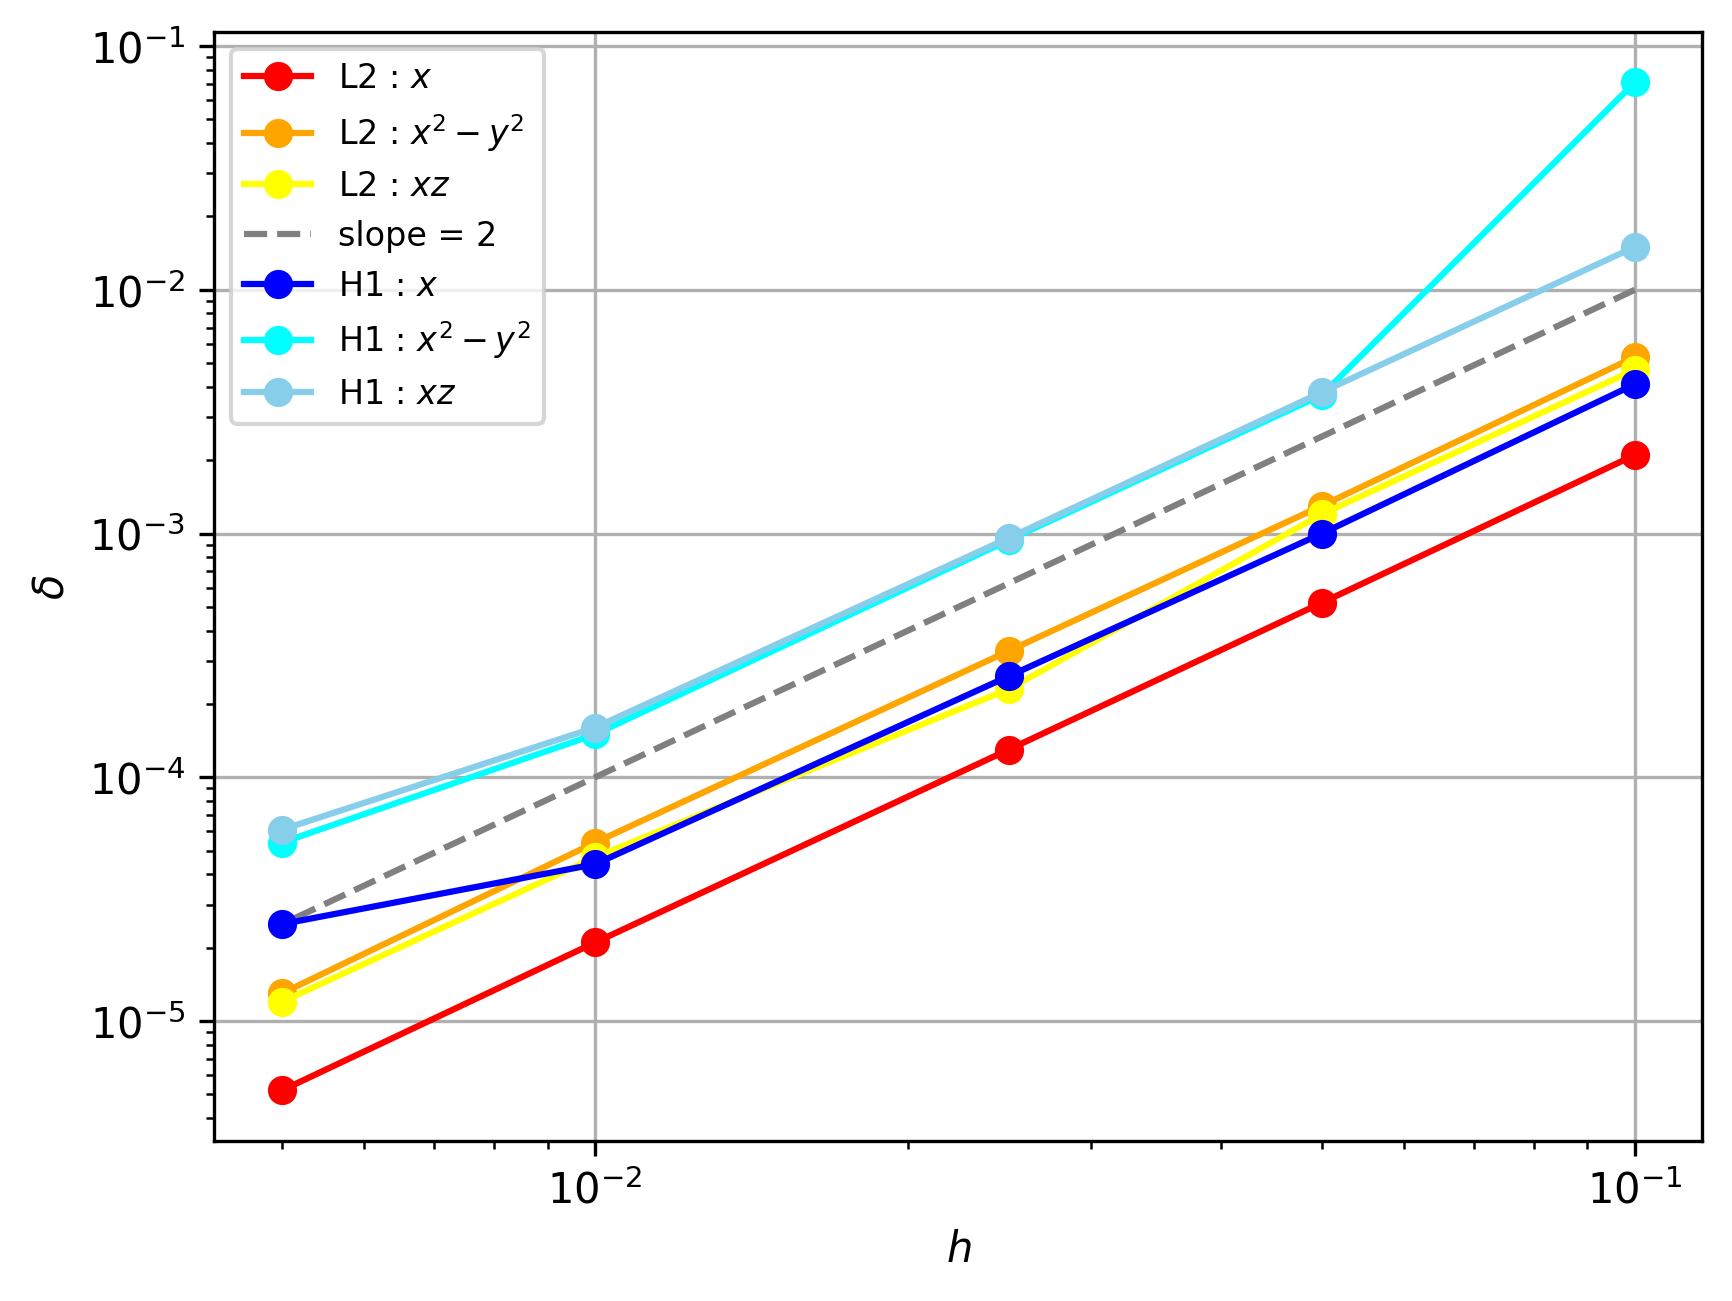
\includegraphics[width=\textwidth]{Errors_P1.png}
         \caption{$L^2$ and $H^1$ norms of the error for $\mathbb{P}_1$}
         \label{fig:errors_p1}
     \end{subfigure}
     \hfill
     \begin{subfigure}[b]{0.48\textwidth}
         \centering
         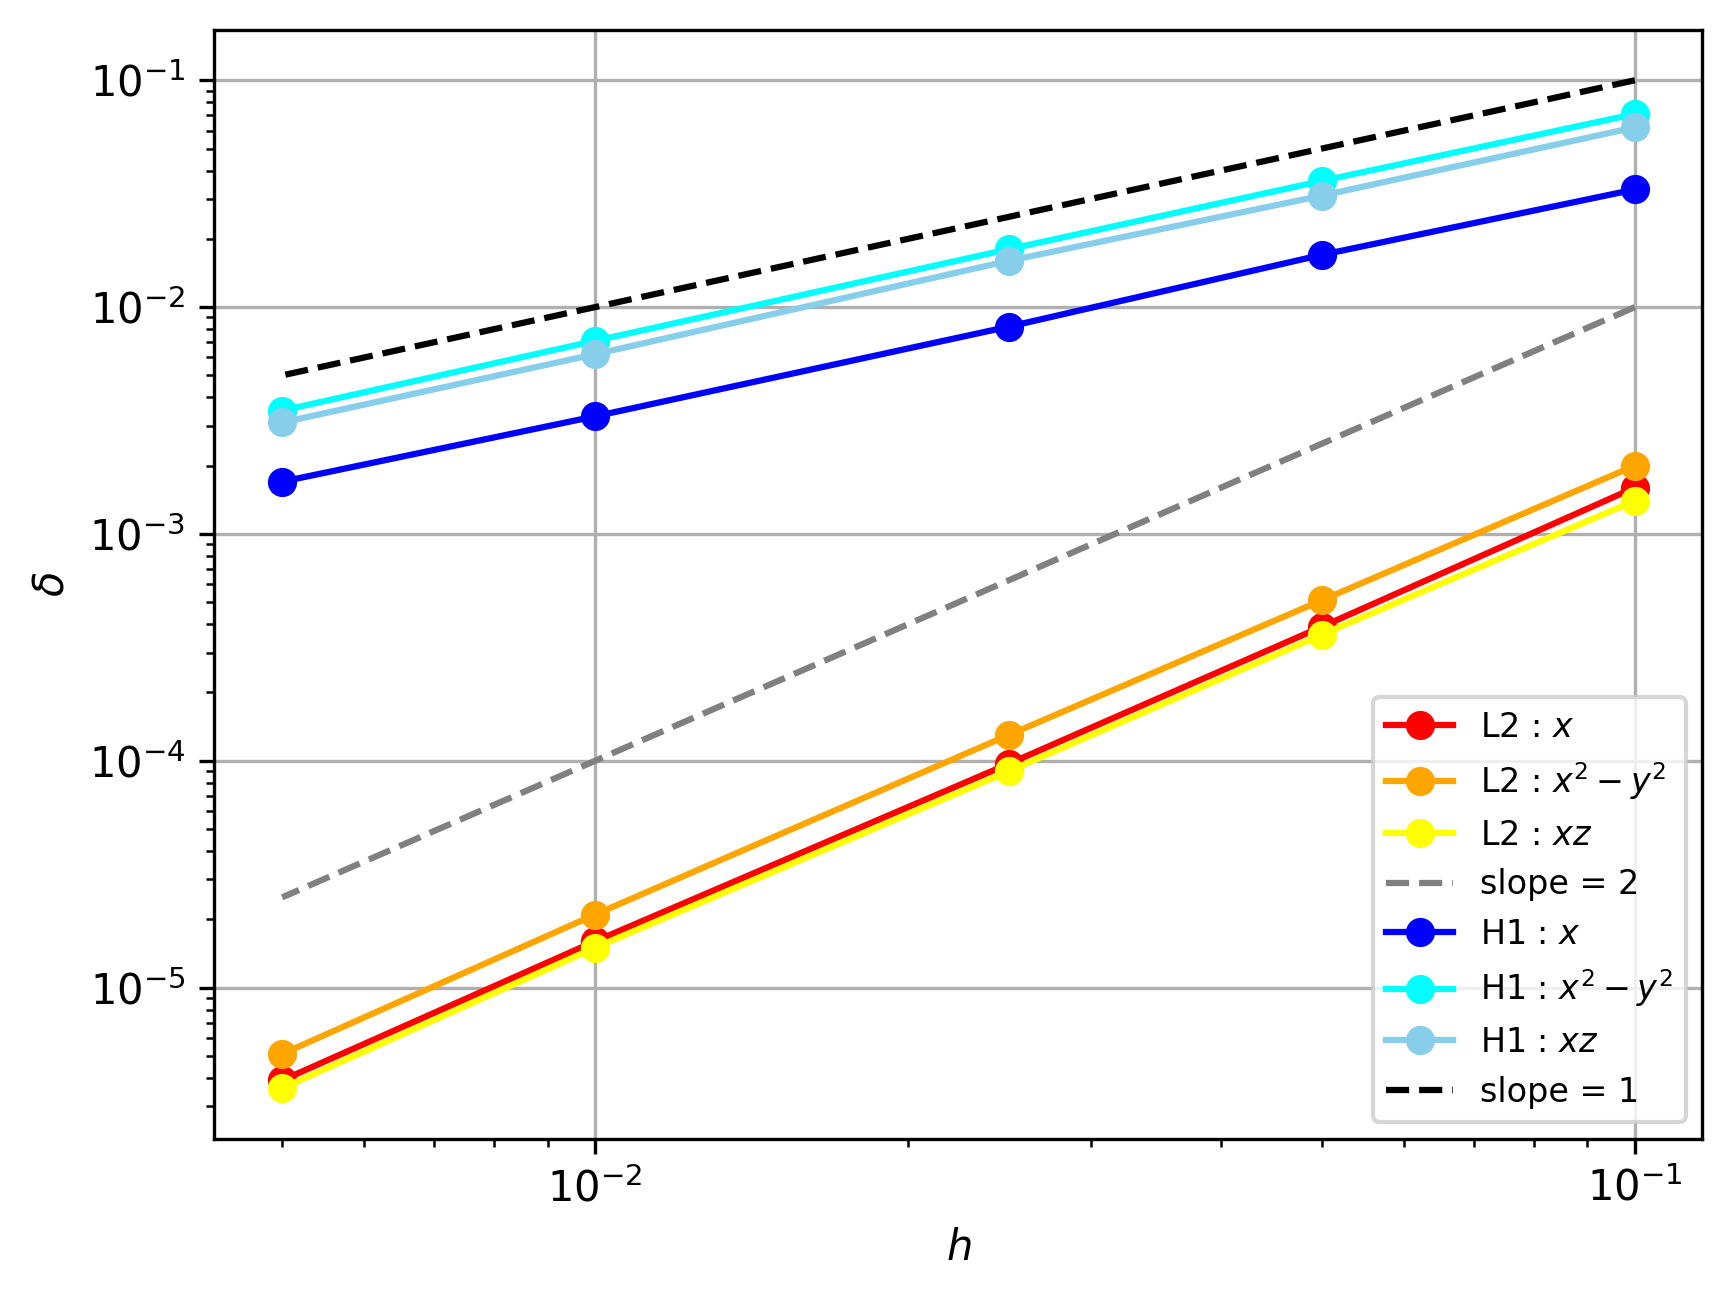
\includegraphics[width=\textwidth]{Errors_P2.png}
         \caption{$L^2$ and $H^1$ norms of the error for $\mathbb{P}_2$}
         \label{fig:errors_p2}
     \end{subfigure}
     \caption{$L^2$ and $H^1$ norms of the error for $\mathbb{P}_1$ et $\mathbb{P}_2$}
     \label{fig:comparison_errors}
\end{figure}

On subplot (a), we recognize the classical $\mathbb{P}_1$ convergence rate in the $L^2$ norm, which is $O(h^2)$. However, we also observe the same convergence rate in the $H^1$ norm, instead of the expected $O(h)$. This is a super-convergence result. \\

On subplot (b), we can see that we have lost one order of convergence compared to the theoretical expectations for $\mathbb{P}_2$. In fact, we observe an $O(h^2)$ rate instead of $O(h^3)$ for the $L^2$ norm, and an $O(h)$ rate instead of $O(h^2)$ for the $H^1$ norm. As mentioned in the project description, this likely stems from the approximation of the sphere by flat triangles.


\subsection{Navier-Stokes solver}

As mentioned at the beginning of this section, we will not test the code as explicitly as we did for the Poisson solver. Instead, we aim to validate the solver by interpreting the results through visualization tools. \\

We recall that we are solving the Navier-Stokes equations in their vorticity-stream function formulation:

$$\partial_t \omega + (\bm \nabla ^{\perp} \psi \cdot \bm \nabla)\omega - \nu \Delta \omega = 0$$

where $\psi$ satisfies the Poisson equation $\Delta \psi = \omega$, with an initial condition $\omega_0$ prescribed by the user. \\

In what follows, we test the code on two different configurations: a viscous flow where diffusion dominates transport, and the inverse case. To do so, we must be able to compare the physical viscosity $\nu$ with other parameters. One approach is to write a non-dimensional version of the equation to highlight a dimensionless number—such as the Reynolds number—that can be used to compare these effects. \\

Let us consider a characteristic vorticity $\bar{\omega}$, stream function $\bar{\psi}$, length $\bar{L}$, and time $\bar{t}$. We define the dimensionless variables $\omega^* = \omega / \bar{\omega}$, $\psi^* = \psi / \bar{\psi}$, $\bm{x}^* = \bm{x} / \bar{L}$, and $t^* = t / \bar{t}$. Introducing the dimensionless operators $\bm{\nabla}^*$ and $\Delta^*$, the equation reads as:

$$\frac{\bar \omega}{\bar t}\partial_{t^*} \omega^* + \frac{\bar \psi \bar \omega}{\bar L^2}(\bm \nabla ^{*\perp} \psi^* \cdot \bm \nabla^*)\omega^* - \frac{\nu \bar \omega}{\bar L^2} \Delta^* \omega^* = 0$$

By choosing the time scale $\bar t = \frac{\bar L^2}{\bar \psi}$, the equation can be rewritten as: 

$$\partial_{t^*} \omega^* + (\bm \nabla ^{*\perp} \psi^* \cdot \bm \nabla^*)\omega^* - \frac{\nu }{\bar \psi} \Delta^* \omega^* = 0$$

There are two regimes: if $\nu \gg \bar \psi$, the viscous term dominates the transport term; conversely, if $\nu \ll \bar \psi$, the transport term dominates the viscous term.

\subsubsection{Viscous flow}

We begin with the case where the viscous term dominates the transport term. This simulation is easily performed by setting a large viscosity, as mentioned above. In order to obtain a clear visual interpretation, we can take the following initial condition:

$$\omega_0(x, y, z) = ze^{-z^2}$$ 

Typically, when running a simulation with $\nu \approx 10^{-1}$, we observe $\bar \psi \approx 10^{-12}$, such that $\nu \gg \bar \psi$. Under these conditions, we obtain the following results:

\begin{figure}[H]
     \centering
     \begin{subfigure}[b]{0.48\textwidth}
         \centering
         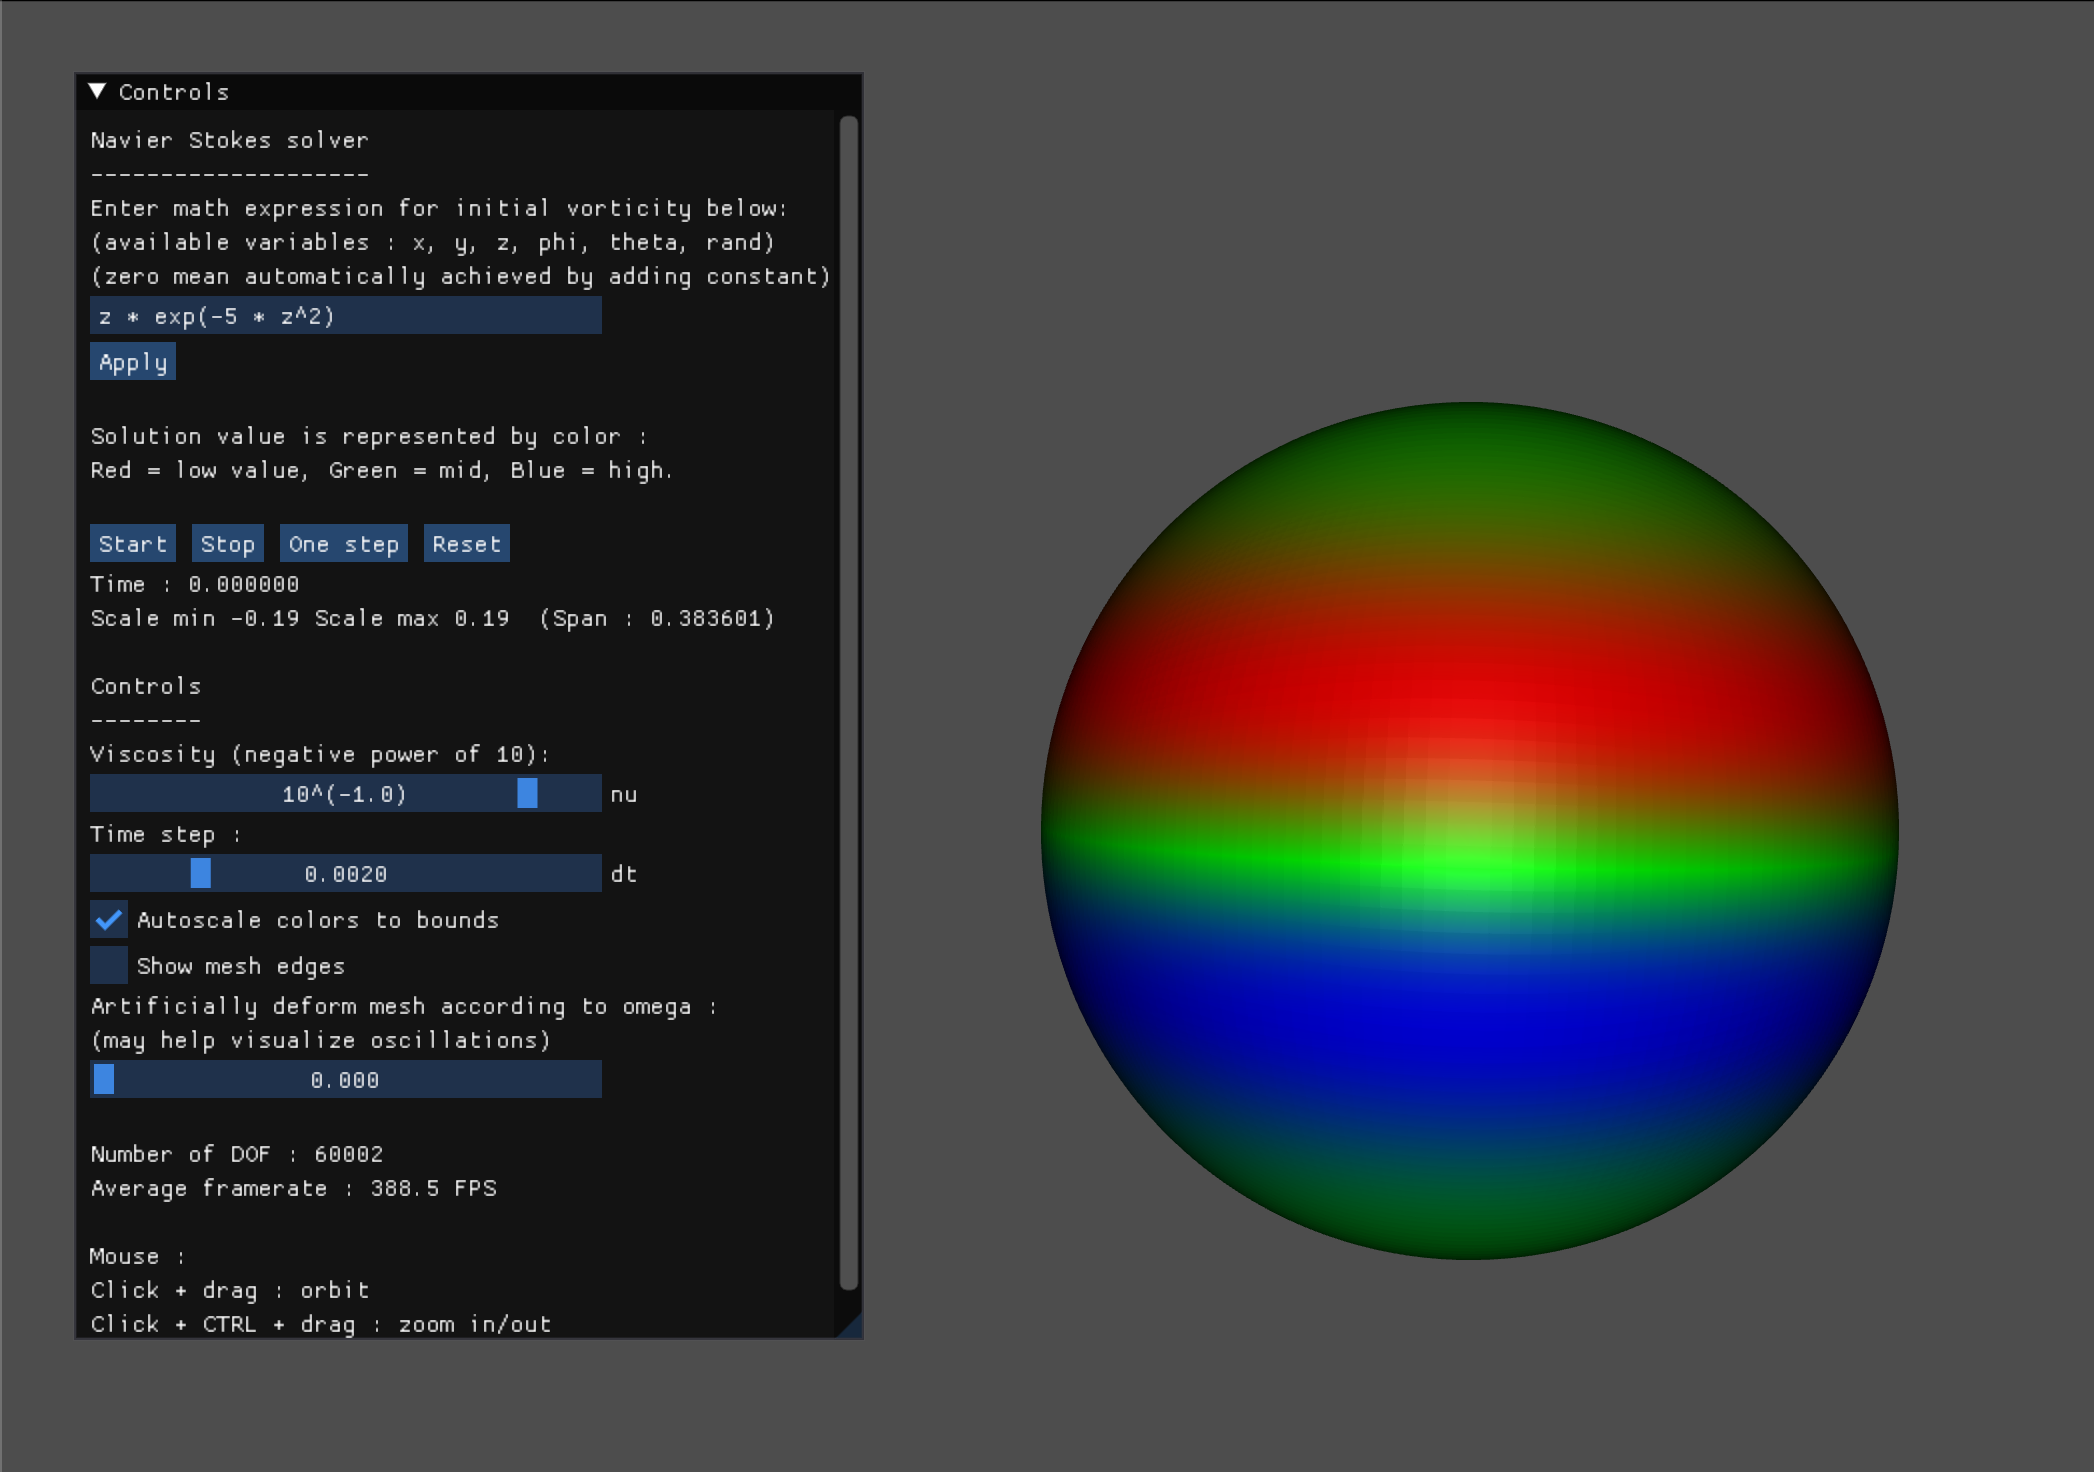
\includegraphics[width=\textwidth]{viscous_init.png}
         \caption{$t = 0$}
         \label{fig:errors_p1}
     \end{subfigure}
     \hfill
     \begin{subfigure}[b]{0.48\textwidth}
         \centering
         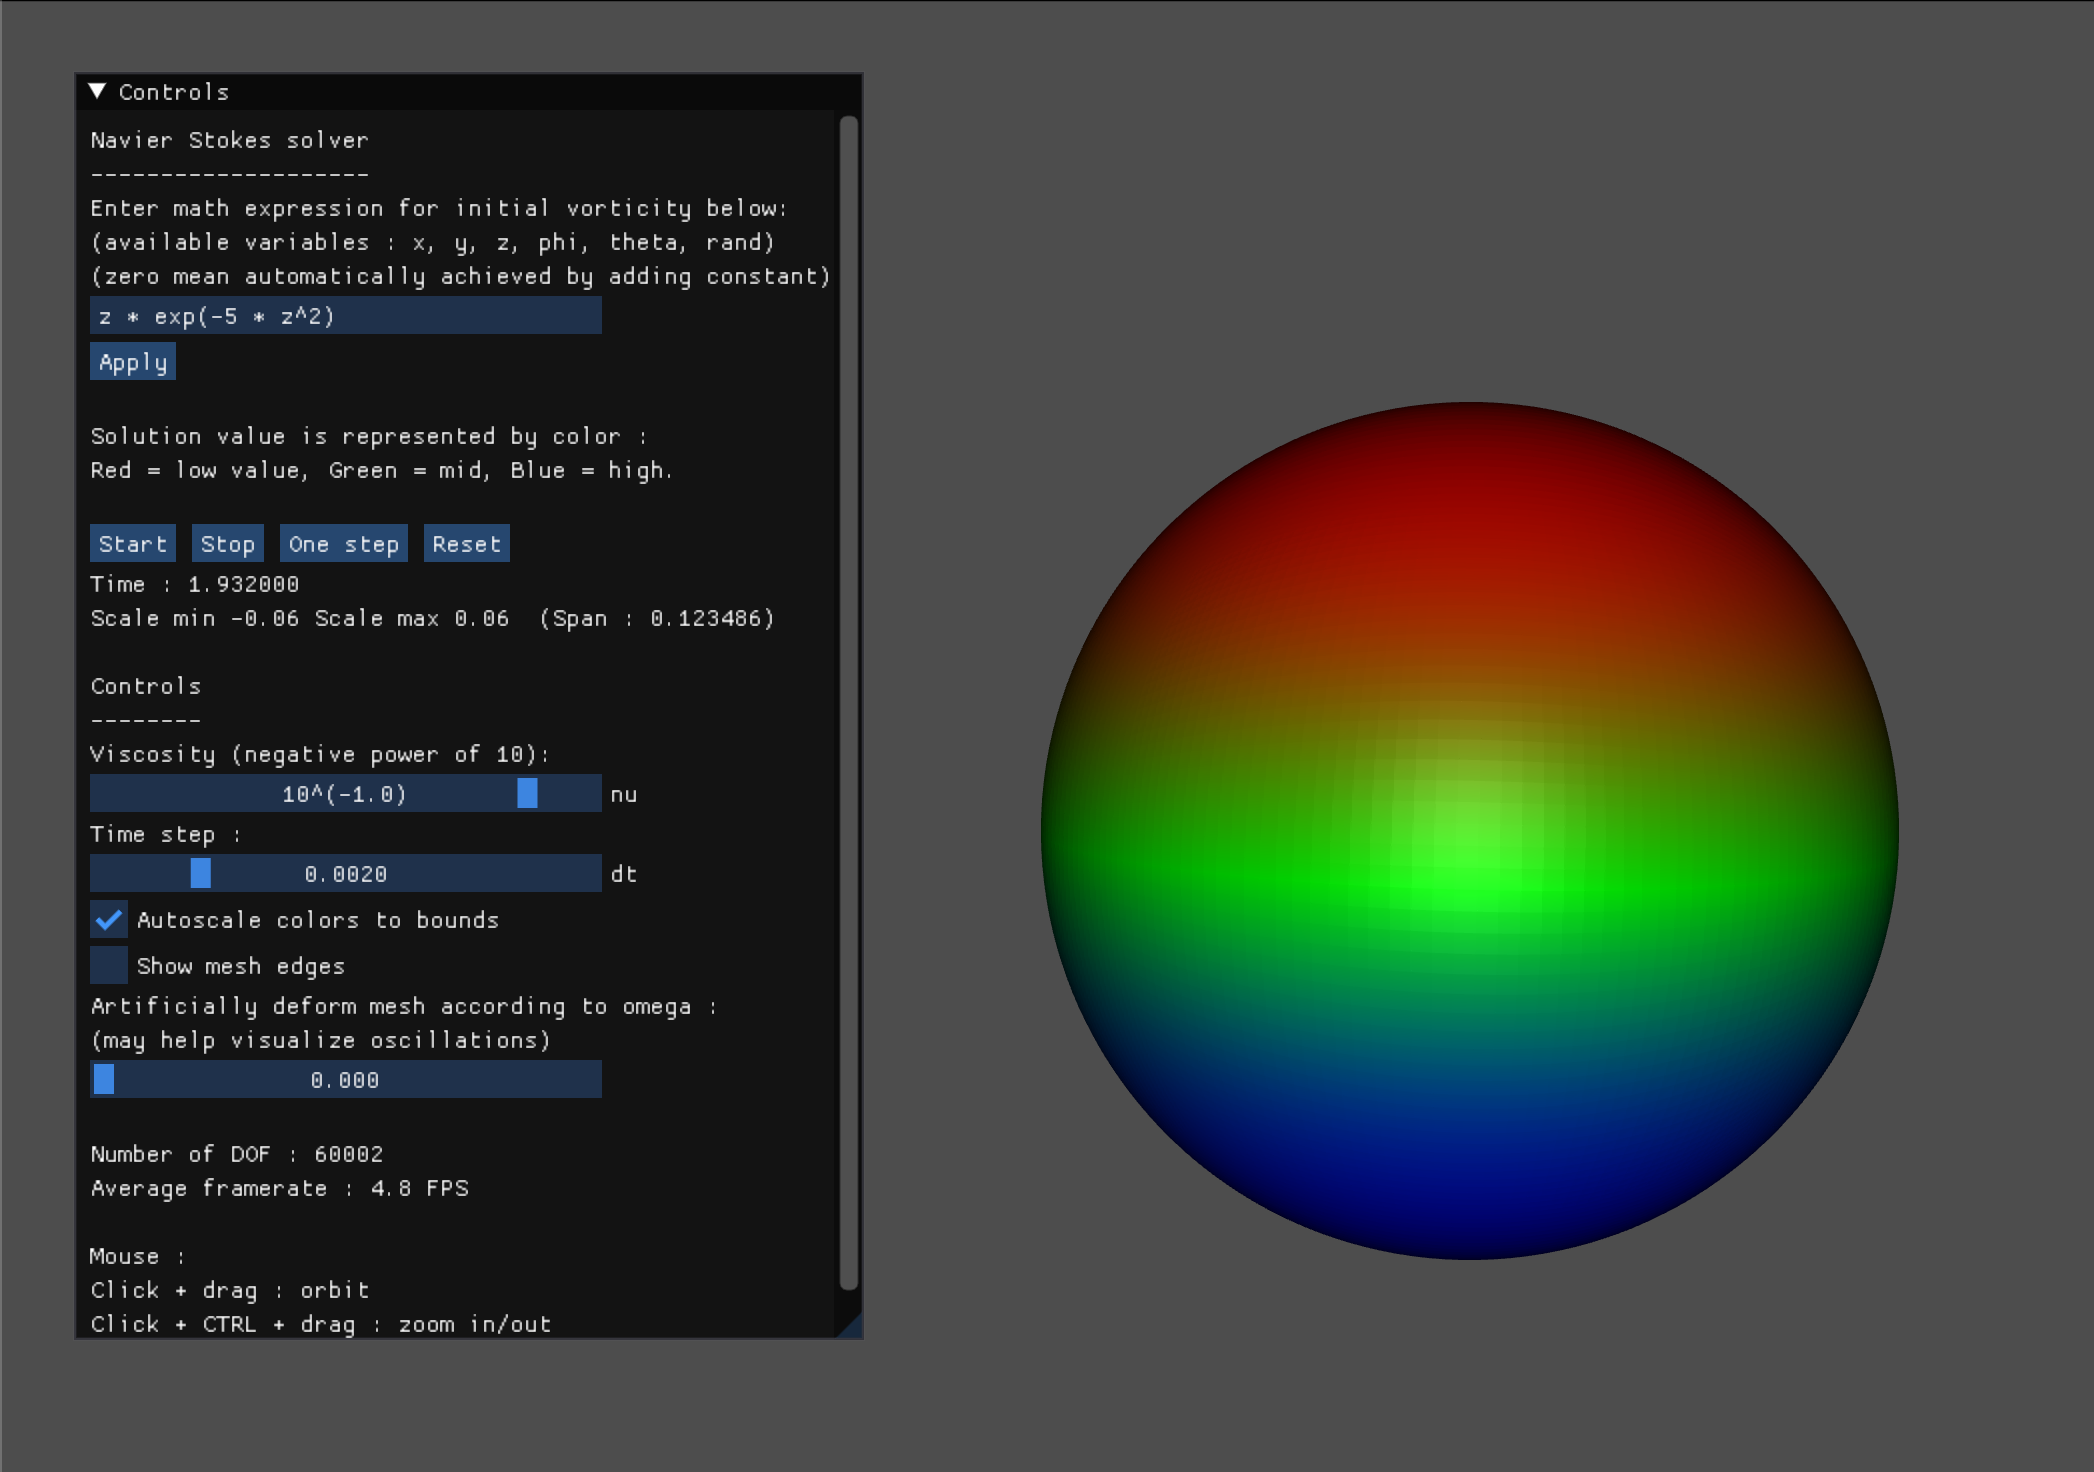
\includegraphics[width=\textwidth]{viscous_end.png}
         \caption{$t = t_f$}
         \label{fig:errors_p2}
     \end{subfigure}
     \caption{Initial and final states of the Navier-Stokes problem with $\nu = 10^{-1}$ and $\omega_0(x, y, z) = ze^{-z^2}$}
     \label{fig:comparison_errors}
\end{figure}

When the viscous effect dominates the transport term, the equation effectively reduces to a diffusion equation on the sphere:

$$\partial_t \omega = \nu \Delta \omega$$

which is equivalent to the heat equation. Given the initial condition, the vorticity diffuses across the sphere. The positive and negative lobes spread toward the north and south poles respectively, much like heat would redistribute. This behavior is clearly illustrated in Figure 3. Eventually, the solution decays to zero over time, as the system lacks a source term to sustain the energy. This mirrors a physical experiment where a sphere is heated at $t=0$ and then left to cool; without a continuous heat source, its temperature eventually equilibrates with its surroundings (zero in our model).

\subsubsection{Transport flow}

Now, we set $\nu \ll \bar{\psi}$ to highlight the behavior of the transport term. This case is more challenging than the previous one because reducing $\nu$ requires a smaller time step to satisfy the CFL (Courant-Friedrichs-Lewy) condition. Consequently, the simulations are slower and can become less stable.\\

After testing several initial conditions and various values for $\nu$, the results remain somewhat unsatisfying, as the simulations consistently develop significant numerical instabilities. However, it is worth noting that the integral of the transport term over the sphere is nearly zero (on the order of $10^{-10}$). This indicates that the computed transport term does not introduce any artificial mass into the system. Furthermore, the $\mathbb{P}_2$ solver demonstrates superior stability compared to the $\mathbb{P}_1$ solver for advection-dominated flows; under identical configurations, the $\mathbb{P}_1$ solver quickly produces \texttt{NaN} values, whereas the $\mathbb{P}_2$ solver maintains a bounded solution where errors accumulate locally without immediate divergence.

\end{document}

